\documentclass[border={7pt 0pt 7pt 0pt},varwidth]{standalone}
\usepackage{amsmath}
\usepackage[dvipsnames]{xcolor}%colors
\usepackage{tikz-cd,tikz-3dplot} 
\usepackage{diagbox}
\usepackage{makecell}
\usepackage{adjustbox}
\usepackage{multirow}
\usepackage[width=0.5,tiewidth=0.7]{strands}
\usepackage{array}


\newcommand{\fakestar}{*}

% https://tex.stackexchange.com/questions/372642/looking-for-symbol-fire
\usepackage{fontspec}
\newfontfamily\emojifont{OpenSansEmoji} % https://github.com/MorbZ/OpenSansEmoji
\DeclareTextFontCommand{\emoji}{\emojifont}
\begin{document}
\begin{table}[]
\arraycolsep=1pt
\[
 \setcellgapes{0ex}\makegapedcells
\begin{array}{ccccccc}
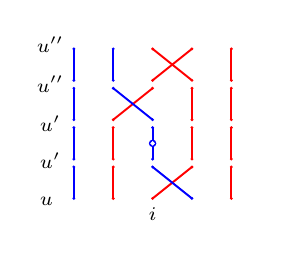
\begin{tikzpicture}[baseline=(current bounding box)]
         \node at (-0.3,0.06) {$\scriptstyle u\phantom{'}$};
         \node at (2.3,0.06) {$\phantom{\scriptstyle u}$};
         \node at (-0.3,0.53) {$\scriptstyle u'$};
         \node at (-0.3,1) {$\scriptstyle u'$};
         \node at (-0.3,1.5) {$\scriptstyle u''$};
         \node at (-0.3,2) {$\scriptstyle u''$};
         \node at (1,-0.15) {$\scriptstyle i$};
         \node at (1.5,-0.15) {$\phantom{\scriptstyle i+1}$};
         \tie[color=blue,bull=1,bulletie=0.01,style=solid]{{1,1.95},{1,1.55}}
         \tie[color=blue,bull=1,bulletie=0.01,style=solid]{{1,1.45},{1,1.05}}
         \tie[color=blue,bull=1,bulletie=0.01,style=solid]{{1,0.95},{1,0.55}}
         \tie[color=blue,bull=1,bulletie=0.01,style=solid]{{1,0.45},{1,0.05}}
         \tie[color=red,bull=1,bulletie=0.01,style=solid]{{4,1.95},{3,1.55}}
         \tie[color=red,bull=1,bulletie=0.01,style=solid]{{3,1.45},{2,1.05}}
         \tie[color=red,bull=1,bulletie=0.01,style=solid]{{2,0.95},{2,0.55}}
         \tie[color=red,bull=1,bulletie=0.01,style=solid]{{2,0.45},{2,0.05}} 
         \tie[color=red,bull=1,bulletie=0.01,style=solid]{{3,1.95},{4,1.55}}
         \tie[color=red,bull=1,bulletie=0.01,style=solid]{{4,1.45},{4,1.05}}
         \tie[color=red,bull=1,bulletie=0.01,style=solid]{{4,0.95},{4,0.55}}
         \tie[color=red,bull=1,bulletie=0.01,style=solid]{{4,0.45},{3,0.05}}
         \tie[color=blue,bull=1,bulletie=0.01,style=solid]{{2,1.95},{2,1.55}}
         \tie[color=blue,bull=1,bulletie=0.01,style=solid]{{2,1.45},{3,1.05}}
         \tie[color=blue,bull=1,bulletie=0.01,style=solid]{{3,0.95},{3,0.55}}
         \tie[color=blue,bull=1,bulletie=0.01,style=solid]{{3,0.45},{4,0.05}}
         \tie[color=red,bull=1,bulletie=0.01,style=solid]{{5,1.95},{5,1.55}}
         \tie[color=red,bull=1,bulletie=0.01,style=solid]{{5,1.45},{5,1.05}}
         \tie[color=red,bull=1,bulletie=0.01,style=solid]{{5,0.95},{5,0.55}}
         \tie[color=red,bull=1,bulletie=0.01,style=solid]{{5,0.45},{5,0.05}}
         \tie[color=blue]{{3,0.75}}\tie[color=white,bulletie=0.02]{{3,0.75}} 
         \end{tikzpicture}
            &=& 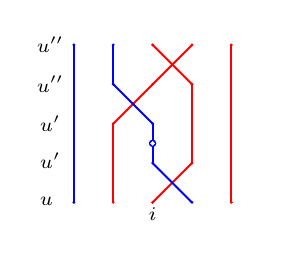
\begin{tikzpicture}[baseline=(current bounding box)]
                 \node at (-0.3,0.06) {$\scriptstyle u\phantom{'}$};
                 \node at (2.3,0.06) {$\phantom{\scriptstyle u'}$};
                 \node at (-0.3,0.53) {$\scriptstyle u'$};
                 \node at (-0.3,1) {$\scriptstyle u'$};
                 \node at (-0.3,1.5) {$\scriptstyle u''$};
                 \node at (-0.3,2) {$\scriptstyle u''$};
                 \node at (1,-0.15) {$\scriptstyle i$};
                 \node at (1.5,-0.15) {$\phantom{\scriptstyle i+1}$};
                 \tie[color=blue,bull=1,bulletie=0.01,style=solid]{{1,2},{1,0}}
                 \tie[color=red,bull=1,bulletie=0.01,style=solid]{{4,2},{3,1.5},{2,1},{2,0}}
                 \tie[color=red,bull=1,bulletie=0.01,style=solid]{{3,2},{4,1.5},{4,0.5},{3,0}}
                 \tie[color=blue,bull=1,bulletie=0.01,style=solid]{{2,2},{2,1.5},{3,1},{3,0.5},{4,0}}
                 \tie[color=red,bull=1,bulletie=0.01,style=solid]{{5,2},{5,0}} \tie[color=blue]{{3,0.75}}\tie[color=white,bulletie=0.02]{{3,0.75}}
                 \end{tikzpicture}
        &\hspace{10mm}$\,$
        &
    \begin{tikzpicture}[baseline=(current bounding box)]
    \node at (-0.3,0.06) {$\scriptstyle u\phantom{'}$};
    \node at (2.3,0.06) {$\phantom{\scriptstyle u}$};
    \node at (-0.3,0.43) {$\scriptstyle u'$};
    \node at (-0.3,0.83) {$\scriptstyle u\phantom{'}$};
    \node at (-0.3,1.2) {$\scriptstyle u'$};
    \node at (1.5,-0.15) {$\phantom{\scriptstyle i+1}$};
%    \node at (1,0.7) {\textcolor{blue}{\emoji{🔥}}};
    \node at (1.5,0.7) {\textcolor{red}{\emoji{🔥}}};
    \tie[color=blue,bull=1,bulletie=0.01,style=solid]{{1,0.5},{1,0}}
    \tie[color=red,bull=1,bulletie=0.01,style=solid]{{2,0.5},{2,0}}
    \tie[color=red,bull=1,bulletie=0.01,style=solid]{{4,0.5},{3,0}}
    \tie[color=blue,bull=1,bulletie=0.01,style=solid]{{3,0.5},{4,0}}
    \tie[color=red,bull=1,bulletie=0.01,style=solid]{{5,0.5},{5,0}} 
    \tie[color=blue,bull=1,bulletie=0.01,style=solid]{{1,1.2},{1,0.7}}
    \tie[color=red,bull=1,bulletie=0.01,style=solid]{{2,1.2},{2,0.7}}
    \tie[color=red,bull=1,bulletie=0.01,style=solid]{{4,1.2},{3,0.7}}
    \tie[color=blue,bull=1,bulletie=0.01,style=solid]{{3,1.2},{4,0.7}}
    \tie[color=red,bull=1,bulletie=0.01,style=solid]{{5,1.2},{5,0.7}}
    \end{tikzpicture}        &=&
    0
           \\
\multicolumn{3}{c}{D_3^{u,u'} \fakestar(e_{3}^{u'})^{-1} \fakestar D_2^{u',u''} \fakestar D_3^{u'',u''}} &&\multicolumn{3}{c}{D_3^{u,u'} \fakestar D_3^{u,u'}=0}
\end{array}
\]
\end{table}

\end{document}